%; whizzy paragraph -pdf xpdf -latex ./whizzypdfptex.sh
%; whizzy-paragraph "^\\\\begin{frame}\\|\\\\emtext"
% latex beamer presentation.
% platex, latex-beamer でコンパイルすることを想定。 

%     Tokyo Debian Meeting resources
%     Copyright (C) 2012 Junichi Uekawa

%     This program is free software; you can redistribute it and/or modify
%     it under the terms of the GNU General Public License as published by
%     the Free Software Foundation; either version 2 of the License, or
%     (at your option) any later version.

%     This program is distributed in the hope that it will be useful,
%     but WITHOUT ANY WARRANTY; without even the implied warreanty of
%     MERCHANTABILITY or FITNESS FOR A PARTICULAR PURPOSE.  See the
%     GNU General Public License for more details.

%     You should have received a copy of the GNU General Public License
%     along with this program; if not, write to the Free Software
%     Foundation, Inc., 51 Franklin St, Fifth Floor, Boston, MA  02110-1301 USA

\documentclass[cjk,dvipdfmx,12pt]{beamer}
\usetheme{Tokyo}
\usepackage{monthlypresentation}

%  preview (shell-command (concat "evince " (replace-regexp-in-string "tex$" "pdf"(buffer-file-name)) "&")) 
%  presentation (shell-command (concat "xpdf -fullscreen " (replace-regexp-in-string "tex$" "pdf"(buffer-file-name)) "&"))
%  presentation (shell-command (concat "evince " (replace-regexp-in-string "tex$" "pdf"(buffer-file-name)) "&"))

%http://www.naney.org/diki/dk/hyperref.html
%日本語EUC系環境の時
\AtBeginDvi{\special{pdf:tounicode EUC-UCS2}}
%シフトJIS系環境の時
%\AtBeginDvi{\special{pdf:tounicode 90ms-RKSJ-UCS2}}

\newenvironment{commandlinesmall}%
{\VerbatimEnvironment
  \begin{Sbox}\begin{minipage}{1.0\hsize}\begin{fontsize}{8}{8} \begin{BVerbatim}}%
{\end{BVerbatim}\end{fontsize}\end{minipage}\end{Sbox}
  \setlength{\fboxsep}{8pt}
% start on a new paragraph

\vspace{6pt}% skip before
\fcolorbox{dancerdarkblue}{dancerlightblue}{\TheSbox}

\vspace{6pt}% skip after
}
%end of commandlinesmall

\title{東京エリアDebian勉強会}
\subtitle{第106回 2013年11月度}
\author{上川純一}
\date{2013年11月16日}
\logo{
\includegraphics[width=8cm]{image200607/openlogo-light.eps}}

\begin{document}

\begin{frame}
\titlepage{}
\end{frame}

\begin{frame}{設営準備にご協力ください。}
会場設営よろしくおねがいします。
\end{frame}

\begin{frame}{Agenda}
 \begin{minipage}[t]{0.45\hsize}
  \begin{itemize}
   \item 注意事項
	 \begin{itemize}
	  \item 飲食禁止
	 \end{itemize}
   \item 最近あったDebian関連のイベント報告
	 \begin{itemize}
	  \item 第103回 東京エリアDebian勉強会
	  \item OSC Tokyo/Fall
	 \end{itemize}
  \end{itemize}
 \end{minipage} 
 \begin{minipage}[t]{0.45\hsize}
  \begin{itemize}
   \item Debian Trivia Quiz
   \item 事前課題紹介
  \end{itemize}
 \end{minipage}
\end{frame}

\section{イベント報告}
\emtext{イベント報告}

\begin{frame}{第103回 東京エリアDebian勉強会}
\end{frame}

\begin{frame}{OSC Tokyo Fall}
\end{frame}

\section{Debian Trivia Quiz}
\emtext{Debian Trivia Quiz}
\begin{frame}{Debian Trivia Quiz}

  Debian の常識、もちろん知ってますよね?
知らないなんて恥ずかしくて、知らないとは言えないあんなことやこんなこと、
みんなで確認してみましょう。

今回の出題範囲は\url{debian-devel-announce@lists.debian.org},
\url{debian-devel@lists.debian.org} に投稿された
内容などからです。

\end{frame}

\subsection{問題}
 %; whizzy-master ../debianmeetingresume201311.tex
% $B0J>e$N@_Dj$r$7$F$$$k$?$a!"$3$N%U%!%$%k$G(B M-x whizzytex $B$9$k$H!"(Bwhizzytex$B$,MxMQ$G$-$^$9!#(B
%

\santaku
{alioth $B$K$J$K$,$*$-$?$+(B}
{$B7|>^$,$"$?$C$?(B}
{RAID$B$N%O!<%I%G%#%9%/$,(B2$B8D2u$l$?(B}
{$B?7%"!<%-%F%/%A%c$K0\9T$7$?(B}
{B}
{RAID$B$N%O!<%I%G%#%9%/$,(B2$B$D2u$l$F%U%!%$%k%7%9%F%`$,2u$l$?$=$&$G$9!#(B}

\santaku
{DSA$B$,(BDPL$B$N>5G'$J$/;H$($kM=;;$O$$$/$i$+(B}
{\$ 0}
{\$ 100}
{\$ 400}
{C}
{$B%G%#%9%/$,2u$l$F8r49$9$k$N$K$b(BDPL$B$r$^$?$J$$$H$$$1$J$+$C$?$N$+$J!#(B}

\santaku
{Jessie $B$N%U%j!<%:$O$$$D$+(B}
{2013$BG/(B11$B7n(B5$BF|(B}
{2014$BG/(B11$B7n(B5$BF|(B}
{2015$BG/(B11$B7n(B5$BF|(B}
{A}
{$B$"$l!"$b$&%U%j!<%:$7$F$k!)(B}

\santaku
{policy 3.9.5.0$B$K$h$k$H%P%$%J%j%Q%C%1!<%8Fb$N%U%!%$%kL>$N%(%s%3!<%G%#%s%0$O$J$K$+(B}
{UTF-8}
{Latin-1}
{sjis}
{A}
{$B$H$&$H$&(BASCII$B0J30$,G'$a$i$l$k$h$&$K$J$j$^$7$?$+!#(B}


\section{事前課題}
\emtext{事前課題}

{\footnotesize
 
\begin{prework}{ $BLn<s(B }

$B8eH/$G$"$j$J$,$iM%0L@-$N$_$i$l$J$$(BMir$B$K0UL#$,$"$k$H$9$l$P!"$=$l$O(BCanonical$B$,%3%s%H%m!<%k2DG=$JE@$@$1$J$N$+$J$H$$$&5$$,$7$^$9!#(B

\end{prework}

\begin{prework}{ dictoss($B?yK\!!E5=<(B) }


\end{prework}

\begin{prework}{  $B@6LnM[0l(B }

$BIaCJ$"$^$j0U<1$7$?$3$H$,$J$+$C$?$N$G!"$3$l$r5$$KJY6/$G$-$l$P$H;W$$$^$9!#(B
\end{prework}

\begin{prework}{ mtoshi }

$B$5$C$Q$jJ,$+$j$^$;$s(B($BN^(B)
\end{prework}

\begin{prework}{ $B$^$($@$3$&$X$$(B }

$BL>A0$7$+<*$K$7$?$3$H$,$J$$$N$G!"$5$C$Q$jJ,$+$i$J$$!#(B
\end{prework}

\begin{prework}{ $BLnEg!!5.1Q(B }

wayland$B$b4hD%$C$?!*(Bmir$B$O<+J,$O$h$/$o$+$i$s$,!"4hD%$C$F$k!*(BX$B$bIi$1$F$J$$!*(B
$B$$$d!<!"$3$A$i$N@o$$$OL\$,$O$J$;$^$;$s%M!<!#2?;v$b6%AhAj<j$,$$$k$C$FNI$$$3$H$G$9%M!<!#(B
mir$B$H$NHf3S$O8!F$$7$?$3$H$J$$$N$G!"0c$$$K$D$$$FC/$+$h$m$7$/$*$M$,$$$7$^$9!#$$$:$l$K$7$F$b!"<+J,$H$7$F$O!"AH$_9~$_4^$a$F4JC1$KM7$Y$=$&$@$7!"Cf?H$9$C$4$$$o$+$j$d$9$$<BAu$G$"$k!"(Bwayland$B$H$7$P$i$/5:$l$h$&$H;W$C$F$^$9!#(B

$B"((Bmir$B$OD4$Y$F$J$$$h(B?

\end{prework}

\begin{prework}{ $B>e@n=c0l(B }

x11$B$N%W%m%H%3%k$O2~NI$NM>CO$,$"$k$H;W$&$N$G4hD%$C$F3+H/$,?J$_6%Ah$,$"$k$N$O9%$^$7$$$H;W$$$^$9!#(B
\end{prework}

}

\section{wayland}
\emtext{wayland}

\section{tramp}
\emtext{tramp}

\begin{frame}{}
 
emacs つかってますか?

tramp つかってますか?

リモートのファイル管理どうしてますか? sshfs ? git ? screen+emacs ? 

\end{frame}

\begin{frame}{\texttt{/sshx:hostname:path/to/file}}

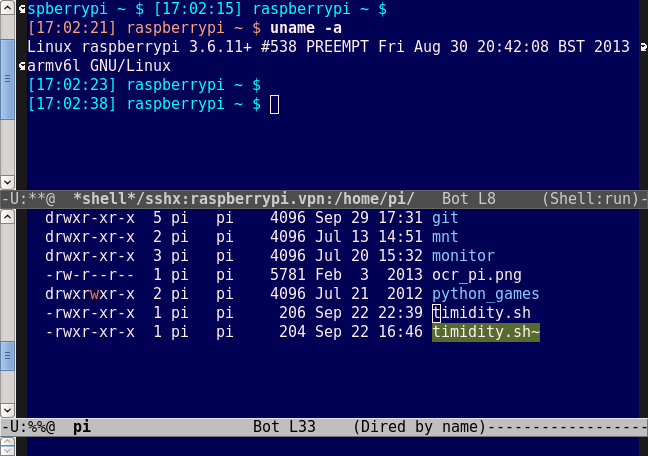
\includegraphics[width=\hsize]{image201311/tramp-screenshot.png}
 
\end{frame}

\begin{frame}{trampのよいところ}
sshでつながるなら
\begin{itemize}
 \item ファイルがひらける
 \item ディレクトリをdiredで操作できる
 \item M-x compile で make がリモートで実行できる
 \item M-x shell などでリモートのシェルを実行できる、かつコマンドがロー
       カルで編集できる
\end{itemize} 
\end{frame}

\begin{frame}{リモート側の設定}

\texttt{.bashrc}を整理

ssh でログインできるように
 
\end{frame}

\begin{frame}[containsverbatim]{\texttt{.ssh/config}}
\begin{commandline}
 ControlMaster auto
 ControlPersist 120
 ControlPath ~/tmp/ssh-%r@%h:%p
\end{commandline}
\end{frame}

\begin{frame}[containsverbatim]{\texttt{.ssh/config}}
\begin{commandline}
 ServerAliveInterval 3
 ServerAliveCountMax 5
\end{commandline}
\end{frame}

\begin{frame}[containsverbatim]{\texttt{.ssh/config}}
\begin{commandline}
 Host *.local
  CheckHostIP no
\end{commandline}
\end{frame}

\begin{frame}[containsverbatim]{\texttt{.ssh/config}}
\begin{commandline}
 Host tekitouna.vpn
  Hostname そのホストのIPアドレス
  IdentityFile ~/.ssh/ssh-keygenで作ったファイルのパス
  IdentitiesOnly yes
\end{commandline}
\end{frame}

\begin{frame}[containsverbatim]{\texttt{.emacs}}
\begin{commandline}
 (add-to-list 'tramp-default-proxies-alist
      '("\\.local\\'" "\\`root\\'" "/ssh:%h:"))
 (custom-set-variables '(tramp-verbose 1))
\end{commandline}
\end{frame}

\section{今後のイベント}
\emtext{今後のイベント}
\begin{frame}{今後のイベント}
\begin{itemize}
 \item 2013年12月 Debian勉強会
\end{itemize}
\end{frame}

\section{今日の宴会場所}
\emtext{今日の宴会場所}
\begin{frame}{今日の宴会場所}
未定
\end{frame}

\end{document}

;;; Local Variables: ***
;;; outline-regexp: "\\([ 	]*\\\\\\(documentstyle\\|documentclass\\|emtext\\|section\\|begin{frame}\\)\\*?[ 	]*[[{]\\|[]+\\)" ***
;;; End: ***
